\documentclass{article}


% if you need to pass options to natbib, use, e.g.:
 \PassOptionsToPackage{numbers, compress}{natbib}
% before loading neurips_2025


% ready for submission
% \usepackage{neurips_2025}


% to compile a preprint version, e.g., for submission to arXiv, add add the
% [preprint] option:
\usepackage[preprint]{neurips_2025}


% to compile a camera-ready version, add the [final] option, e.g.:
%     \usepackage[final]{neurips_2025}


% to avoid loading the natbib package, add option nonatbib:
%    \usepackage[nonatbib]{neurips_2025}

\setcitestyle{square}
\usepackage[utf8]{inputenc} % allow utf-8 input
\usepackage[T1]{fontenc}    % use 8-bit T1 fonts
\usepackage{hyperref}       % hyperlinks
\usepackage{url}            % simple URL typesetting
\usepackage{booktabs}       % professional-quality tables
\usepackage{amsfonts}       % blackboard math symbols
\usepackage{nicefrac}       % compact symbols for 1/2, etc.
\usepackage{microtype}      % microtypography
% \usepackage{xcolor}         % colors
\usepackage{enumitem}
\usepackage{graphicx}
\usepackage{multirow}
\usepackage[table]{xcolor}
% \usepackage[margin=1in]{geometry}
\usepackage{tabularx}      % 可伸缩列宽
\usepackage{ragged2e}      % 灵活对齐
\usepackage{fontawesome}
\def\hflogowidth{1.5cm}
\def\gitlogowidth{1.2cm}
\title{GraphRAG-Bench: Challenging\\ Domain-Specific Reasoning for Evaluating\\ Graph Retrieval-Augmented Generation}


% The \author macro works with any number of authors. There are two commands
% used to separate the names and addresses of multiple authors: \And and \AND.
%
% Using \And between authors leaves it to LaTeX to determine where to break the
% lines. Using \AND forces a line break at that point. So, if LaTeX puts 3 of 4
% authors names on the first line, and the last on the second line, try using
% \AND instead of \And before the third author name.

% \author{%
%   Yilin Xiao\footnotemark[1]\\
%   The Hong Kong Polytechnic University\\
%   \texttt{yilin.xiao@connect.polyu.hk} \\
%   \And
%   Junnan Dong\footnotemark[1] \footnotemark[2]\\
%   Tencent Youtu Lab \\
%   \texttt{hansonjdong@tencent.com} \\
%   \AND
%   Chuang Zhou \\
%   The Hong Kong Polytechnic University \\
%   \texttt{chuang-qqzj.zhou@connect.polyu.hk} \\
%   \And
%   Su Dong \\
%   The Hong Kong Polytechnic University \\
%   \texttt{su.dong@connect.polyu.hk} \\
%   \And
%   Qian-Wen Zhang \\
%   Tencent Youtu Lab \\
%   \texttt{cowenzhang@tencent.com} \\
%   \And
%   Di Yin \\
%   Tencent Youtu Lab \\
%   \texttt{endymecyyin@tencent.com} \\
%   \And
%   Xing Sun \\
%   Tencent Youtu Lab \\
%   \texttt{winfredsun@tencent.com} \\
%   \And
%   Xiao Huang \\
%   The Hong Kong Polytechnic University \\
%   \texttt{xiao.huang@polyu.edu.hk} \\
% }
\author{%
   \textbf{Yilin Xiao}\textsuperscript{$1 *$},
   \textbf{Junnan Dong}\textsuperscript{$2 *\dag$},\\
   \textbf{Chuang Zhou}\textsuperscript{$1$},
   \textbf{Su Dong}\textsuperscript{$1$},
   \textbf{Qian-Wen Zhang}\textsuperscript{$2$},
   \textbf{Di Yin}\textsuperscript{$2$},
   \textbf{Xing Sun}\textsuperscript{$2$}, 
   \textbf{Xiao Huang}\textsuperscript{$1$}
   \\ 
   $^1$ The Hong Kong Polytechnic University \\ 
   $^2$ Tencent Youtu Lab \\ 
   \texttt{yilin.xiao@connect.polyu.hk, hansonjdong@tencent.com}\\
}

\begin{document}
\renewcommand{\thefootnote}{\fnsymbol{footnote}}
\footnotetext[1]{Equal contribution}
\footnotetext[2]{Corresponding author}

\maketitle


\begin{abstract}
% Graph Retrieval Augmented Generation (GraphRAG) has been increasingly recognized for its potential to enhance large language models (LLMs) by leveraging the structured knowledge in the large corpus. However, current evaluations of GraphRAG models predominantly rely on traditional question-answering datasets. Their limited scope in questions and evaluation metrics fails to comprehensively assess the reasoning capacity improvements enabled by GraphRAG models. To address this gap, we present GraphRAG-Bench, the first challenging domain-specific benchmark with a tailored dataset and a comprehensive evaluation particularly designed for assessing GraphRAG. Specifically, \((i)\) we propose a college-level dataset spanning 16 disciplines, requiring the model to do multi-hop conceptual reasoning, complex algorithm\&programming and mathematical computing. This dataset also features diverse question types, including multiple-choice, true/false, multi-select, open-ended, and fill-in-blank. \((ii)\) GraphRAG-Bench provides a multi-dimensional evaluation of GraphRAG models, assessing the entire pipeline from graph construction, knowledge retrieval to the final generation stage. Crucially, our evaluation framework is designed to provide insights to quantify the underlying LLM's reasoning ability when augmented with structured knowledge. Extensive experiments on nine contemporary GraphRAG methods demonstrate the utility in revealing the impact of graphs on improving model generation and reasoning performance, providing insights to the wider community.
Graph Retrieval Augmented Generation (GraphRAG) has garnered increasing recognition for its potential to enhance large language models (LLMs) by structurally organizing domain-specific corpora and facilitating complex reasoning. However, current evaluations of GraphRAG models predominantly rely on traditional question-answering datasets. Their limited scope in questions and evaluation metrics fails to comprehensively assess the reasoning capacity improvements enabled by GraphRAG models. To address this gap, we introduce GraphRAG-Bench, a large-scale, domain-specific benchmark designed to rigorously evaluate GraphRAG models. Our benchmark offers three key superiorities: \((i)\) Challenging question design. Featuring college-level, domain-specific questions that demand multi-hop reasoning, the benchmark ensures that simple content retrieval is insufficient for problem-solving. For example, some questions require mathematical reasoning or programming. \((ii)\) Diverse task coverage. The dataset includes a broad spectrum of reasoning tasks, multiple-choice, true/false, multi-select, open-ended, and fill-in-the-blank. It spans 16 disciplines in twenty core textbooks. \((iii)\) Holistic evaluation framework. GraphRAG-Bench provides comprehensive assessment across the entire GraphRAG pipeline, including graph construction, knowledge retrieval, and answer generation. Beyond final-answer correctness, it evaluates the logical coherence of the reasoning process. By applying nine contemporary GraphRAG methods to GraphRAG-Bench, we demonstrate its utility in quantifying how graph-based structuring improves model reasoning capabilities. Our analysis reveals critical insights about graph architectures, retrieval efficacy, and reasoning capabilities, offering actionable guidance for the research community. All the related resources of GraphRAG-Bench are collected in \faGithub: \textcolor{blue}{\url{https://github.com/jeremycp3/GraphRAG-Bench}}.




%1.not leverage
%2.
%prof Huang
% Graph Retrieval Augmented Generation (GraphRAG) has garnered increasing recognition for its potential to enhance large language models (LLMs) by structurally organizing domain-specific corpora and facilitating complex reasoning. However, current evaluations of GraphRAG models predominantly rely on traditional question-answering datasets. Their limited scope in questions and evaluation metrics fails to comprehensively assess the reasoning capacity improvements enabled by GraphRAG models. To address this gap, we introduce GraphRAG-Bench, a large-scale, domain-specific benchmark designed to rigorously evaluate GraphRAG models. Our benchmark offers three key contributions:
%\((i)\) Challenging question design. Featuring college-level, domain-specific questions that demand multi-hop reasoning, the benchmark ensures that simple content retrieval is insufficient for problem-solving. For example, some questions require mathematical reasoning or programming. \((ii)\) Diverse task coverage. The dataset includes a broad spectrum of reasoning tasks, multiple-choice, true/false, multi-select, open-ended, and fill-in-the-blank. There are 1018 questions covering topics in twenty textbooks. \((iii)\) Holistic evaluation framework. GraphRAG-Bench provides comprehensive assessment across the entire GraphRAG pipeline, including graph construction, knowledge retrieval, and answer generation. Beyond final-answer correctness, it evaluates the logical coherence of the reasoning process. By applying nine contemporary GraphRAG methods to GraphRAG-Bench, we demonstrate its utility in quantifying how graph-based structuring improves model performance. Our analysis reveals critical insights into the interplay between graph architectures, retrieval efficacy, and reasoning capabilities, offering actionable guidance for the research community.

%original
% Graph Retrieval Augmented Generation (GraphRAG) has been increasingly recognized for its potential to enhance large language models (LLMs) by leveraging the structured knowledge in the large corpus. However, current evaluations of GraphRAG models face a significant gap. They merely rely on datasets for traditional QA, which only contain limited question complexity and a narrow range of question types. This fails to reflect how the integration of graphs influences the reasoning capabilities of these models. To this end, we present GraphRAG-Bench, the first challenging domain-specific benchmark with a tailored dataset and a comprehensive evaluation particularly designed for assessing GraphRAG. Specifically, \((i)\) we propose a college-level dataset spanning 16 disciplines, requiring the model to do multi-hop conceptual reasoning, complex algorithm\&programming and mathematical computing. This dataset also features diverse question types, including multiple-choice, true/false, multi-select, open-ended, and fill-in-blank. \((ii)\) We offer a multi-dimensional evaluation of GraphRAG models, assessing the entire pipeline from graph construction, knowledge retrieval to the final generation stage. Crucially, our evaluation framework is designed to provide insights to quantify the underlying LLM's reasoning ability when augmented with structured knowledge. Extensive experiments on nine contemporary GraphRAG methods demonstrate the utility in revealing the impact of graphs on improving model generation and reasoning performance, providing insights to the wider community.


\end{abstract}

\section{Introduction}
Retrieval-Augmented Generation (RAG)~\cite{RAG,RAG_survey} has emerged as a key solution to ground large language models (LLMs) in external knowledge to mitigate both the hallucination problem and the lack of domain knowledge. By retrieving relevant text passages from corpora, RAG injects factual knowledge for a more reliable generation from LLMs. However, conventional RAG systems remain unsatisfactory when dealing with complex reasoning scenarios. The flat retrieval in RAG directly returns fragmentized chunks based on similarity matching, which limits their ability to model complex relationships between concepts to answer the questions requiring multi-hop reasoning~\cite{graphrag_survey,dong2023hierarchy}, i.e., `What was the impact of [event] the 2008 Lehman Brothers bankruptcy on [person] Elon Musk's Tesla?' or global comprehension, i.e., `What is the main idea of the [event] Trade Policy Change?'.

To address these limitations, Graph Retrieval-Augmented Generation (GraphRAG) has been extensively studied to capture the structured knowledge among concepts in the form of graphs~\cite{graphrag, graphrag_survey_2,DIGIMON}, where nodes represent concepts and edges are for the relations among them. Recent advances in GraphRAG can be categorized into three main directions. First, hierarchical graph construction methods like RAPTOR~\cite{raptor} and Microsoft's GraphRAG~\cite{graphrag} organize knowledge through tree structures and community detection. Second, neural graph retrieval approaches, including GFM-RAG~\cite{GFM} and G-Retriever~\cite{G-Retriever} employ graph neural encoders with specialized objectives for multi-hop reasoning. Third, dynamic knowledge integration systems such as DALK~\cite{dalk} and ToG~\cite{TOG} develop adaptive graph construction and traversal mechanisms that are tightly coupled with LLMs. By structuring knowledge as graphs, GraphRAG enables LLMs to both traverse and reason over explicit relational paths, but also supports deeper reasoning by inferring implicit relations based on the graph structure. 

\begin{figure*}
    \centering
    
\includegraphics[width=1\linewidth]{figure1.pdf}
    \caption{A sketched overview of our benchmark \texttt{GraphRAG-Bench}, illustrating the contributions.}
    \label{fig:enter-label}
\end{figure*}
%of both dataset and evaluation.
However, despite the promise, existing benchmarks for GraphRAG methods fail to reflect the performance of reasoning on graphs. They predominantly leverage the traditional QA dataset, e.g., HotpotQA~\cite{hotpotqa}, 2WikiMultiHopQA~\cite{2wikimultihop} and MuSiQue~\cite{musique}, which only feature explicit factoid questions with limited complexity and short answers, e.g., `Who is the grandchild of Dambar Shah?'.  These datasets suffer from three critical limitations: \((i)\) There are only commonsense questions that could be probably covered in the training corpus of LLMs. \((ii)\) They typically require only single-hop or shallow multi-hop reasoning based on explicit connections, which inadequately probes the unique advantages of graph-structured knowledge.  \((iii)\) Narrow Answer Formats. Most answers are short (names, dates) or multiple-choice, which could hardly reflect the reasoning ability over graphs. To this end, we would like to ask a research question:

\textit{\textbf{``Does graph augmentation truly enhance reasoning capabilities beyond simple retrieval?''}}
%is it necssary to build a graph 

In this paper, we propose GraphRAG-Bench, the first challenging domain-specific benchmark particularly designed for GraphRAG. \((i)\) Our dataset contains $1$,$018$ college-level question spans 16 disciplines, e.g., computer vision, computer networks, human-computer interaction, AI ethics, etc, featuring the ability of conceptual understanding, e.g., ``Given [theorem] A and B, prove [conclusion] C'', complex algorithmic programming, e.g., coding with interlinked function calls) and mathematical computation, e.g., ``Given [Input], [Conv1], [MaxPool], [FC], calculate the output volume dimensions.'' \((ii)\) GraphRAG-Bench contains five types of diverse questions to thoroughly evaluate different aspects of reasoning, including multiple-choice (MC), multi-select (MS), true-or-false (TF), fill-in-blank (FB) and open-ended (OE).  \((iii)\) We offer a comprehensive multi-dimensional evaluation on each component of GraphRAG, including graph construction, knowledge retrieval, answer generation and rationale generation. We aim to provide unprecedented insights into how graph-structured knowledge enhances LLMs' reasoning capabilities compared to traditional RAG approaches. The major contributions are summarized hereunder:

% Overall, we propose the first challenging domain-specific benchmark, particularly concentrating on GraphRAG. It contains $1$,$018$ questions in 5 question types spanning 16 topics and a corpus of 7 million words from 20 computer science textbooks. A comprehensive evaluation protocol is designed to stress-test GraphRAG methods on graph construction, retrieval, and multi-hop answer generation and rationale generation. Extensive experiments have been conducted with nine state-of-the-art GraphRAG models. We make insightful observations and provide the insights that: 1) GraphRAG substantially enhances the reasoning capabilities of LLMs, and - to the best of our knowledge - we are the first to quantify this improvement using concrete evaluation metrics.  2) GraphRAG’s impact varies by question types: it yields significant gains on some types but offers limited benefit for others.

\textbf{Contributions:}
\begin{itemize}[leftmargin=*]
    \item We propose the first challenging domain-specific benchmark, particularly concentrating on GraphRAG. It contains 1018 questions in 5 question types spanning 16 topics and a corpus of 7 million words from 20 computer science textbooks;
    \item A comprehensive evaluation protocol is designed to stress-test GraphRAG methods on graph construction, retrieval, and multi-hop answer generation and rationale generation.
    \item Extensive experiments have been conducted with nine state-of-the-art GraphRAG models. We make insightful observations and provide the insights that: 1) GraphRAG substantially enhances the reasoning capabilities of LLMs, and - to the best of our knowledge - we are the first to quantify this improvement using concrete evaluation metrics.  2) GraphRAG’s impact varies by question types: it yields significant gains on some types but offers limited benefit for others.
\end{itemize}

\section{Related Work}
\textbf{GraphRAG.} Recent work in GraphRAG has focused on integrating structured knowledge and advanced retrieval strategies to overcome the limitations of vanilla RAG in handling large, noisy corpora and complex reasoning. For example, RAPTOR~\cite{raptor} and Microsoft’s GraphRAG~\cite{graphrag} both employ hierarchical clustering, RAPTOR via recursive tree construction with multi-level summarization, and GraphRAG via community detection with LLM-generated synopses, to support coarse-to-fine retrieval and diverse, high-coverage responses. GFM-RAG~\cite{GFM}, G-Retriever~\cite{G-Retriever}, and LightRAG~\cite{lightrag} each combine graph neural encoders with specialized retrieval objectives, respectively a query dependent GNN trained in two stages for multi-hop generalizability, a Prize Collecting Steiner Tree formulation to reduce hallucination and improve scalability, and a dual level graph augmented index for efficient, incrementally updatable lookup, to enable accurate, scalable reasoning over document graphs. Inspired by hippocampal memory processes, HippoRAG~\cite{hippo} leverages Personalized PageRank to achieve single-step multi-hop retrieval, delivering state-of-the-art efficiency and performance on both path following and path finding QA tasks. DALK~\cite{dalk} and KGP~\cite{KGP} introduce dynamic KG construction and traversal agents, using LLMs to build domain specific graphs and self aware retrieval policies, to inject structural context while reducing noise. ToG~\cite{TOG} tightly couples LLMs with KGs via beam search exploration, enabling iterative graph reasoning and on the fly correction without additional training. Collectively, these methods exemplify the GraphRAG paradigm by uniting graph structures, generative language models, and novel retrieval formulations to enhance knowledge integration, scalability, and deep reasoning across diverse domains.
% Recent work in GraphRAG has focused on integrating structured knowledge and advanced retrieval strategies to overcome the limitations of vanilla RAG in handling large, noisy corpora and complex reasoning. For example, RAPTOR~\cite{raptor} and Microsoft's GraphRAG~\cite{graphrag} both employ hierarchical clustering—RAPTOR via recursive tree construction with multi-level summarization, and GraphRAG via community detection with LLM-generated synopses—to support coarse-to-fine retrieval and diverse, high-coverage responses. GFM-RAG~\cite{GFM}, G-Retriever~\cite{G-Retriever}, and LightRAG~\cite{lightrag} each combine graph neural encoders with specialized retrieval objectives—respectively a query-dependent GNN trained in two stages for multi-hop generalizability, a Prize-Collecting Steiner Tree formulation to reduce hallucination and improve scalability, and a dual-level graph-augmented index for efficient, incrementally updatable lookup—to enable accurate, scalable reasoning over document graphs. Inspired by hippocampal memory processes, HippoRAG~\cite{hippo} leverages Personalized PageRank to achieve single-step multi-hop retrieval, delivering state-of-the-art efficiency and performance on both path-following and path-finding QA tasks. DALK~\cite{dalk} and KGP~\cite{KGP} introduce dynamic KG construction and traversal agents—using LLMs to build domain-specific graphs and self-aware retrieval policies—to inject structural context while reducing noise. ToG~\cite{TOG} tightly couples LLMs with KGs via beam-search exploration, enabling iterative graph reasoning and on-the-fly correction without additional training. 


\textbf{Prior benchmarks for GraphRAG.} To date, no dataset has been specifically designed for GraphRAG tasks. Widely used datasets such as Quality~\cite{quality}, PopQA~\cite{popqa}, and HotpotQA~\cite{hotpotqa} are tailored for general question answering, where answers can often be directly extracted from corpora, failing to effectively measure the core capabilities of GraphRAG methods. Multi-hop QA datasets like MusiqueQA~\cite{musique} and 2WikiMultiHopQA~\cite{2wikimultihop} contain questions artificially constructed via rules and logic, rather than natural queries from real-world scenarios. Additionally, their corpora are short and often derived from converting entities and descriptions of existing KGs, which deviates from practical application contexts. While DIGIMON~\cite{DIGIMON} benchmarks some methods, it neither introduces new datasets nor evaluates the reasoning capabilities of GraphRAG. Critically, all aforementioned datasets neglect question type distinctions, focusing primarily on simple questions and thus unable to reflect GraphRAG's performance variations across different question categories. In summary, existing datasets lack long contexts and raw documents, mismatching real-world scenarios, and omit gold rationale, making it impossible to systematically evaluate GraphRAG's reasoning abilities.

\section{GraphRAG-Bench: Challenging Reasoning Benchmark for GraphRAG} 
\subsection{Question design}
To evaluate the GraphRAG framework on college-level reasoning, we first assembled an authoritative textbook corpus. Beginning with over 100 publications spanning 16 distinct subfields in computer science, we systematically identified the most representative 20 textbooks. We defined five types of questions, each targeting a different aspect of GraphRAG's reasoning capabilities, which are detailed in Tab.~\ref{question_type}. After rigorous screening and refinement by several domain experts, we selected 1,018 high-quality challenging questions, covering a broad spectrum of topics.

By design, each question type is explicitly mapped to the core competencies of GraphRAG, with individual questions meticulously crafted for application in college-level instructional or assessment contexts. Should GraphRAG demonstrate improved performance on these tasks, it would establish itself as a highly effective tool in education, significantly enhancing teaching and learning efficiency.

\begin{table}[htbp]
\centering
\begin{tabularx}{\linewidth}{lX}
\toprule
\textbf{Question Type} & \textbf{Description} \\
\midrule
Fill-in-blank (FB) & Requires completing context-dependent statements with semantically precise terms. These assess the model’s ability to generate contextually coherent content by leveraging local semantic dependencies and entity grounding within graph-structured knowledge. \\
\addlinespace
Multi-choice (MC) & Presents a question with 4 options, including linguistically plausible distractors. These assess the model’s capacity to discern correct answers through discriminative reasoning, integrating entity information and edge relationships to reject semantically similar but factually incorrect options. \\
\addlinespace
Multi-select (MS) & Demands selecting 2–4 correct answers from 4 options, often requiring reasoning over interconnected concepts. The inclusion of overlapping distractors tests the model’s ability to handle complex query semantics, aggregating evidence from multi-hop graph paths and resolving conflicts between related but non-essential attributes. \\
\addlinespace
True-or-false (TF) & Involves verifying the correctness of statements. These measure the model’s factual accuracy assessment, requiring logical inference over knowledge. \\
\addlinespace
Open-ended (OE) & OE questions allow for a wide range of responses, requiring methods to formulate detailed and comprehensive answers. These evaluate the model’s holistic knowledge synthesis, demanding the integration of multi-subfield knowledge to generate structured, logically coherent long-form responses. \\
\bottomrule
\end{tabularx}
\caption{The description of different question types.}
\label{question_type}
\end{table}

\subsection{Corpus collection and processing}
Extracting accurate content from the 20 PDF-format core textbooks presents significant challenges. We implement a multi-stage pipeline comprising preprocessing, content parsing, post-processing, and hierarchy construction. 

\textbf{Textbook Preprocessing.} 1) PDF Classification: To distinguish text-based pages from scanned (image-based) pages, we analyze each page’s text density and image area proportion. Text-based pages are processed by extracting text directly using PyMuPDF, while scanned pages require optical character recognition (OCR) to extract their textual content.
2) Metadata Extraction: We extract metadata for each textbook, including its outline, total page count, and the page ranges for each chapter or section. This metadata supports the later construction of the document’s logical structure.

\textbf{Content Parsing.} After preprocessing, we analyze each page’s layout to extract textual and non-textual elements.
1) Layout Analysis: We apply LayoutLMv3~\cite{LayoutLMv3} for multimodal document layout analysis. LayoutLMv3 is pre-trained with masked language modeling, masked image modeling, and cross-modal alignment, enabling it to learn rich representations of document pages. The model classifies page regions into semantic categories such as titles, paragraphs, figures, tables, or decorative/irrelevant elements. This segmentation yields coherent content blocks on each page.
2) Formula Recognition: Mathematical formulas embedded in text are often misrecognized by OCR. To prevent this, we first detect inline formulas using a pre-trained YOLO-based model~\cite{Yolo} from PDF-Extract-Kit. This model identifies the bounding boxes of formula regions so that formula images can be extracted separately, ensuring that OCR does not garble the formula content.
3) OCR: In scanned PDFs, OCR is applied to recognize text regions. We use PaddleOCR to transcribe text from the regions labeled as titles and body paragraphs via layout analysis. This step produces the page’s textual content in the correct reading order, while preserving non-text elements as separate objects.


\textbf{Post-Processing.} After parsing, the extracted elements (text blocks, formula, figures, tables, etc.) may be disordered due to overlapping bounding boxes or fragmented text lines. We resolve these issues by reordering and merging page regions according to human reading order. Concretely, we use MinerU~\cite{MinerU} for post-processing, which partitions each page into logical reading regions and sequences them so that the final text flow matches the natural reading sequence.

\textbf{Hierarchy Construction.} Finally, we organize the extracted content into a hierarchical textbook-tree structure. We map the textbook metadata (e.g., chapter titles, section divisions, and page ranges) to a four-level hierarchy: Book Title → Chapter → Section (Subchapter) → Knowledge Content Unit. Each node in this hierarchy is annotated with its contextual metadata and its structural role. This textbook-tree provides an intuitive, pedagogical navigation framework aligned with the textbook’s organization. The resulting corpus – with its accurate content extraction, structural annotation, and hierarchical organization – forms a robust basis for evaluating GraphRAG’s ability to leverage organized textbook knowledge for context-rich reasoning and retrieval-augmented generation.
\subsection{Expert-crafted rationale}
Existing benchmarks typically supply only final answers or explicit graph paths; by contrast, our dataset supplies expert-crafted rationales that articulate the complete logical progression necessary to solve each problem. These rationales go beyond mere corpus aggregation; they are structured narratives that (i) isolate prerequisite concepts, (ii) describe the relationships among these concepts, and (iii) specify the inferential operations applied during problem solving. By tracing each step of logical inference and knowledge interaction, we can assess whether GraphRAG models truly generate contextually grounded explanations or simply exploit surface-level patterns.

To enable fine-grained, topic-specific evaluation, each question in our dataset carries two hierarchical labels: a broad subfield (Level 1, e.g., ``Machine Learning'') and a more granular concept (Level 2, e.g., ``Unsupervised Learning''). These annotations structure our post-hoc analyses. For each topic, we measure not only the accuracy of the model’s answer but also the degree to which its generated rationale aligns with the gold one. In this way, we convert evaluation into a multidimensional process, requiring models to produce both correct solutions and faithful reasoning patterns.

\section{Experiments}
We conduct experiments on each submodule following GraphRAG's pipeline, which includes the \textbf{graph construction} (or similar specialized structures), \textbf{knowledge retrieval}, and \textbf{generation}. Additionally, since our dataset contains a gold rationale for each query, we require the GraphRAG method to generate \textbf{rationales} during the generation phase to evaluate its reasoning capabilities.

\textbf{Metrics.} We provide a succinct introduction to the core ideas of each metric; the full evaluation protocol and details can be found in the Appendix.
\begin{itemize}[leftmargin=*] 
    \item \textbf{Graph construction.} We evaluate graph construction across three aspects: 1) Efficiency: the time required to build a complete graph. 2) Cost: the number of tokens consumed during graph construction. 3) Organization: the proportion of non-isolated nodes within the constructed graph.
    \item \textbf{Knowledge retrieval.} We evaluate retrieval from two dimensions: 1) indexing time, defined as the duration required to construct the vector database for retrieval; 2) average retrieval time, representing the mean time consumed for knowledge retrieval per query. Additionally, we summarize the retrieval operators employed by each method to assess the complexity of their retrieval mechanisms.    
    \item \textbf{Generation.} We argue that the existing exact match metric is inappropriate, as correct answering does not necessitate word-by-word correspondence. Therefore, this paper introduces a new metric, Accuracy, defined as follows: 1) For OE and FB questions, both the generated output and groundtruth are fed into an LLM via our designed prompt, which assigns a score based on semantic alignment and correctness. 2) For MC and TF, 1 point for the correct answer, 0 points for otherwise. 3) For MS, 1 point for a fully correct answer; 0.5 points for a subset; 0 points for incorrect answers.
    \item \textbf{Rationale.} We designed a prompt to feed both the rationale generated by the GraphRAG method and the gold rationale into a LLM, which assigns a reasoning score R to evaluate their semantic correspondence and reasoning consistency. Simultaneously, we developed an additional assessment metric, namely the AR metric, to determine whether the model is able to provide correct reasoning when it answers the question accurately. This metric serves to distinguish whether the model has merely guessed the correct answer or has actually engaged in proper logical reasoning to reach the correct answer, thereby offering a more comprehensive understanding of the model's performance.
\end{itemize}

\textbf{Experiment setups.} In our experiments, we evaluated the performance of nine state-of-the-art GraphRAG methods, including: 1) RAPTOR~\cite{raptor}; 2) LightRAG~\cite{lightrag}; 3) GraphRAG~\cite{graphrag}; 4) G-Retriever~\cite{G-Retriever}; 5) HippoRAG~\cite{hippo}; 6) GFM-RAG~\cite{GFM}; 7) DALK~\cite{dalk}; 8) KGP~\cite{KGP}; 9) ToG~\cite{TOG}. To ensure a fair comparison across all methods, we adopted the same GPT-4o-mini as the default large language model. We imposed no max token length to limit the performance of individual methods. For methods requiring top-k selection, we uniformly set k=5. Regarding text chunking, the chunk size was consistently set to 1200 tokens. Except for the parameters standardized for fair comparison, all other hyperparameters were configured to the optimal values reported in the original papers. 
% All methods were implemented in Python and executed on the same GPUs.
% and the same BGE-M3 as the embedding model during implementation
\subsection{Evaluation of graph construction}

\begin{table}[h]
\resizebox{\linewidth}{!}{%
\begin{tabular}{lccc}
\hline
Method      & Token cost of graph construction & Time cost of graph construction & Organization \\ \hline
RAPTOR (2024)      &           10,142,221            &             20396.49s      &   -           \\
KGP (2024)         &           15,271,633            &              17318.07s      &         46.03\%    \\
LightRAG (2024)    &           83,909,073             &            12976.22s        &  69.71\%           \\
GraphRAG (2025)    &           79,929,698             &            11181.24s        &  72.51\%          \\
G-Retriever (2024) &           32,948,161             &            5315.27s       & 89.95\%          \\
HippoRAG (2024)   &           33,006,198             &            5051.41s        & 89.58\%           \\
% HippoRAG v2 &                                  &                         &         0.74\%    \\
DALK (2024)       &           33,007,324             &            \textbf{4674.30s}      &  89.49\%           \\
ToG (2024)       &           33,008,230             &             5235.30s       &       89.95\%   \\
GFM-RAG (2025)    &           32,766,094             &            5631.10s      &  \textbf{89.97\%}          \\ \cline{1-4} 
\end{tabular}}
\caption{Comparison of graph construction process.}
\label{graph}
\end{table}
% \vspace{-10pt}
Graph construction aims to transform corpus into structured, storable objects, serving as the foundational step in GraphRAG. Current mainstream graph construction methods can be categorized into four classes: 1) Tree: RAPTOR leverages this structure, where each leaf node represents a chunk. By generating summaries via LLMs and applying clustering methods, parent nodes are iteratively created to form a hierarchical tree structure. 2) Passage Graph: Adopted by KGP, this structure represents each chunk as a node, with edges established through entity linking tools. 3) Knowledge Graph: Used in G-Retriever, HippoRAG, GFM-RAG, and DALK, this structure extracts entities and relationships from chunks using open information extraction (OpenIE) tools to construct knowledge graphs. 4) Rich Knowledge Graph: Employed by GraphRAG and LightRAG, this structure enriches standard knowledge graphs with additional information (e.g., summarizing descriptions for nodes or edges).

Experimental results in Tab.~\ref{graph} show that the tree structure incurs the lowest token count, as it only invokes LLMs for summary generation, but requires the longest time due to iterative clustering. The passage graph has suboptimal token cost, invoking LLMs only for summarizing entities or relationships, with the second-longest time consumption attributed to the time-intensive entity linking process. The knowledge graph has moderate token usage, requiring LLMs for both entity extraction from corpora and triple generation from entities, yet achieves the shortest time consumption due to rapid knowledge graph construction after triple acquisition. The rich knowledge graph consumes the most tokens, as it generates additional descriptions for entities and relationships via LLMs on top of standard knowledge graphs, leading to increased time costs. For evaluating graph construction quality, we use the non-isolated nodes ratio as the metric. Since the Tree structure contains no isolated nodes, this metric is inapplicable to it. Experimental results show that the Knowledge Graph achieves the best performance, with its non-isolated nodes ratio maintained at approximately 90\%. The Rich Knowledge Graph performs suboptimally; while it incorporates additional information, it inevitably introduces more noise. The Passage Graph exhibits the lowest non-isolated nodes ratio, indicating that entity linking tools fail to effectively establish edges between most entity pairs.

\subsection{Evaluation of knowledge retrieval}

As shown in Tab. \ref{retrieval}. GFM-RAG incurs the shortest indexing time; it does not construct a traditional vector database to store entities but instead stores question-corresponding entities exclusively during graph construction. Among methods using vector databases, KGP, RAPTOR, and DALK exhibit lower costs due to minimal stored information; ToG, G-Retriever, and LightRAG have moderate costs, as relationship storage is inherently time-consuming; GraphRAG further increases indexing time by additionally storing community reports. HippoRAG demands the longest indexing time, attributed to its extra construction of entity<->relationship and relationship<->chunk mappings.
Regarding average retrieval time, RAPTOR achieves the fastest speed, as its tree structure enables rapid information localization. GFM-RAG and HippoRAG follow, leveraging GNNs and PageRank algorithms for retrieval, respectively. G-retriever employs a prize-collecting Steiner forest algorithm, while LightRAG relies on relationship-based retrieval, both introducing additional latency. GraphRAG needs to utilize community information for retrieval, which leads to its time-consuming. KGP, ToG, and DALK incur substantial time costs due to their dependence on LLM invocations during retrieval.

\begin{table}[htbp]
\resizebox{\linewidth}{!}{%
\begin{tabular}{lccc}
\hline
Method      & Retrieval operators               & Indexing time & Average retrieval time \\ \hline
% HippoRAG v2 & Node+Relationship+Chunk           &               &                        \\
KGP         & Node                              &    204.10s      &  89.38s                 \\
ToG         & Node+Relationship                 &    1080.43s    &   70.53s                \\ 
GraphRAG    & Node+Relationship+Chunk+Community &   1796.65s    &    44.87s                   \\
DALK        & Node+Subgraph                     &   407.10s         & 26.80s                       \\
G-Retriever & Node+Relationship+Subgraph        &    920.39s     &    23.77s                  \\
LightRAG    & Node+Relationship+Chunk           &   1430.32s      &  13.95s                      \\
HippoRAG    & Node+Relationship+Chunk           &   4695.29s      &   2.44s                   \\
GFM-RAG     & Node           &     \textbf{93.55s}       &     1.96s                   \\
RAPTOR      & Node                              &   451.03s            &  \textbf{0.02s}                      \\\hline
\end{tabular}}
\caption{Comparison of knowledge retrieval process.}
\label{retrieval}
\end{table}
% \vspace{-20pt}
\subsection{Evaluation of generation accuray}

\begin{table}[h]
\centering
\resizebox{\linewidth}{!}{%
\begin{tabular}{lcccccc}
\hline
\multirow{2}{*}{Method} & \multicolumn{6}{c}{Accuracy}     \\ \cline{2-7} 
                        & Fill-in-blank & Multi-choice & Multi-select & True-or-false  & Open-ended & Average \\ \hline
\rowcolor{gray!20} GPT-4o-mini    &   74.29 &  81.11  &  76.68  &  75.95  &  52.23  & 70.68  \\ \hline
 TF-IDF    & 75.71 & 77.88 & 72.52 &  84.17  & 50.18 &  71.71$\uparrow$     \\
 BM-25    &  74.28 & 78.80 & 71.17 & \textbf{84.49} & 50.00 &   71.66$\uparrow$  \\\hline
DALK    & 70.00   & 78.34 & 71.62   &  77.22  & 51.49  &  69.30$\downarrow$     \\
G-Retriever    & 70.95 & 77.42 & 71.62 &78.80 & 52.04 &   69.84$\downarrow$  \\
LightRAG    & 65.24 & 78.80 & 73.42  &  82.59 & 53.16   &   71.22$\uparrow$   \\
ToG        & 70.48 & 78.80 &  \textbf{78.38}  & 79.75 &  54.28  &   71.71$\uparrow$  \\ 
KGP       & 74.29 & 79.26 &74.77 &   82.28 & 51.49 &  71.86$\uparrow$   \\
GFM-RAG    & 72.38 & 80.65 & 72.07 & 82.59 & 52.79 &   72.10$\uparrow$    \\
GraphRAG    &  75.24 & \textbf{81.57} & 77.48 & 80.70  &52.42 &   72.50$\uparrow$   \\
HippoRAG     & 70.48 & 80.18 & 74.32 & 81.65 & \textbf{56.13}  &  72.64$\uparrow$   \\
RAPTOR    & \textbf{76.67} & 80.65 & 77.48 & 82.28 &  54.83 & \textcolor{purple}{\textbf{73.58}}$\uparrow$    \\ \hline
\end{tabular}}
\caption{Comparison of generation process.}
\label{generation}
\end{table}
% \vspace{-10pt}
As shown in Tab.\ref{generation}. Given that GPT-4o-mini already exhibits strong question-answering capabilities, not all GraphRAG methods effectively enhance its performance. Notably, DALK and G-Retriever degrade LLM performance; their over-reliance on structural information at the expense of semantic content introduces excessive noise during generation, impairing LLM judgment accuracy. LightRAG, ToG, and KGP achieve slight performance improvements, indicating their retrieved content provides marginal assistance for generation tasks. In contrast, GFM-RAG, GraphRAG, and HippoRAG significantly boost LLM performance by effectively integrating graph structural information with chunk-level semantics: GFM-RAG leverages large-scale pretraining to obtain a robust foundation model, GraphRAG optimizes retrieval using community-based information, and HippoRAG enhances retrieval efficiency via PageRank algorithm. The top-performing method in experiments is RAPTOR, which constructs a tree structure through iterative clustering, a design that aligns with the natural hierarchical organization of textbook data, enabling efficient retrieval of relevant information. Additionally, most GraphRAG methods outperform traditional RAG baselines such as BM-25 and TF-IDF, highlighting the utility of graph-based architectures in improving generation accuray.  

\subsection{Evaluation of reasoning capabilities}
As shown in Tab.\ref{reasoning}. In contrast to the high accuracy in generation tasks, GPT-4o-mini exhibits a notable decline in reasoning performance. The decrease in R score indicates that LLMs often fail to perform correct reasoning, instead selecting answers through conjecture or pattern matching in many cases. The drop in AR score suggests that even when LLMs provide correct answers, their reasoning processes may be flawed; alternatively, they might generate correct reasoning but choose incorrect answers. Importantly, all GraphRAG methods significantly enhance the reasoning capabilities of LLMs: through distinct algorithmic designs, these methods retrieve not only semantically relevant corpus for questions but also identify multi-hop dependent corpus in the knowledge base, providing evidential support for LLM reasoning. This enables LLMs to reason based on external information rather than relying solely on internal knowledge for conjecture. In terms of algorithm performance, the distribution aligns with that of generation tasks: HippoRAG and RAPTOR remain the top performers, which is intuitive, since retrieving useful information is inherently correlated with enabling correct reasoning. Additionally, most GraphRAG methods still outperform traditional RAG baselines.

\begin{table}[htbp]
\resizebox{\linewidth}{!}{%
\begin{tabular}{lcccccccccccc}
\hline
\multirow{3}{*}{Method} & \multicolumn{12}{c}{Reasoning}                                                                                                                                                                                                                                                                                                               \\ \cline{2-13} 
                        & \multicolumn{2}{c}{FB}                                & \multicolumn{2}{c}{MC}                                & \multicolumn{2}{c}{MS}                                & \multicolumn{2}{c}{TF}                                & \multicolumn{2}{c}{OE}                               & \multicolumn{2}{c}{Average}                           \\ \cline{2-13} 
                        & R                         & AR                        & R                         & AR                        & R                         & AR                        & R                         & AR                        & R                         & AR                       & R                         & AR                        \\ \hline
\rowcolor{gray!20}GPT-4o-mini             & \multicolumn{1}{l}{64.76} & \multicolumn{1}{l}{53.33} & \multicolumn{1}{l}{55.07} & \multicolumn{1}{l}{50.92} & \multicolumn{1}{l}{54.50} & \multicolumn{1}{l}{39.19} & \multicolumn{1}{l}{58.23} & \multicolumn{1}{l}{53.40} & \multicolumn{1}{l}{49.26} & \multicolumn{1}{l}{9.76} & \multicolumn{1}{l}{55.45} & \multicolumn{1}{l}{39.78} \\ \hline
TF-IDF             &         68.09         &          52.61         &   52.76                   &    49.19           &        56.30          &      43.02                 &        64.08       &       61.23          &             50.37    &   10.50                   &           57.61       &     42.38   \\
BM-25             &        69.04            &      56.42               &    57.14                  &          53.11           &        57.20              &    42.79                  &         65.18            &        62.18               &               50.74      &         11.52          &      59.18       &    44.15     \\ \hline
DALK                    & 70.95                     & 55.24                     & 54.15                     & 50.35                     & 59.01                     & 46.40                     & 62.18                     & 58.23                     & 54.09                     & 9.67                     & 58.89                     & 42.12                     \\
KGP                     & 64.29                     & 49.29                     & 56.45                     & 52.07                     & 58.11                     & 44.37                     & 64.08                     & 60.68                     & 52.42                     & 8.92                     & 58.74                     & 42.22                     \\
GraphRAG                & \textbf{71.43}                     & 55.24                     & 56.22                     & 52.42                     & 57.66                     & 45.72                     & 63.61                     & 60.13                     & 53.16                     & 10.50                    & 59.43                     & 43.30                     \\
G-Retriever             & 70.00                     & 55.00                     & \textbf{57.60}                     & \textbf{53.46}                     & 60.81                     & 48.20                     & 64.24                     & 60.21                     & 53.35                     & 10.04                    & 60.17                     & 43.66                     \\
LightRAG                & 66.19                     & 47.86                     & 57.14                     & 52.30                     & \textbf{61.71}                     & \textbf{49.10}                     & 66.61                     & 63.45                     & 53.16                     & 10.13                    & 60.46                     & 43.81                     \\
ToG                     & 70.00                     & 53.10                     & 56.00                     & 51.73                     & 57.21                     & 45.72                     & 65.66                     & 62.26                     & 54.46                     & 12.08                    & 60.17                     & 44.01                     \\ 
GFM-RAG                 &         70.00             &         54.76            &          56.22          &          52.07            &         58.11            &            45.50           &         66.46              &       \textbf{63.69}                &           53.72         &         10.69            &       60.36               &     44.30                \\
HippoRAG                & 66.67                     & 50.48                     & 56.68                     & 52.30                     & 59.91                     & 47.52                     & \textbf{67.25}                     & 63.61                     & \textbf{55.02}                     & 12.36                    & \textcolor{purple}{\textbf{60.90}}                    & 44.55                     \\
RAPTOR                  & \textbf{71.43}                     & \textbf{57.86}                     & 56.45                     & 52.07                     & 60.36                     & \textbf{49.10}                     & 66.30                     & 62.90                     & 53.90                     & \textbf{13.57}                    & 60.81                     & \textcolor{purple}{\textbf{45.53}}                     \\ \hline
\end{tabular}}
\caption{Comparison of reasoning ability.}
\label{reasoning}
\end{table}
% \vspace{-20pt}
\subsection{Topic‐specific generation accuracy analysis}

Given our dataset spans 16 distinct topical domains, we conducted a fine‐grained analysis of GraphRAG’s impact on LLM generation accuracy. Overall, GraphRAG yields consistent improvements in most areas; However, several intriguing findings emerge: \textbf{1) Mathematics Domain.} All GraphRAG methods degrade the LLM’s generation accuracy in mathematics. This is attributed to the critical reliance of mathematical problems on rigorous symbolic manipulation and precise reasoning chains; models must internally "compute" each deductive step rather than relying on keyword matching from external texts. Most documents retrieved through GraphRAG are explanatory or conceptual, with symbolic notation, formula layouts, and contextual structures often misaligned with the problem requirements, leading to ambiguities or loss of key steps during the extraction and transformation of information. \textbf{2) Ethics Domain.} Both GraphRAG and the LLM itself exhibit mediocre performance in ethics. We posit that ethical problems fundamentally involve subjective value judgments, whose meanings depend on dynamic contexts of moral trade-offs and social norms. The symbolic representations captured by LLMs through statistical learning struggle to accurately model ambiguous ethical constructs, introducing intrinsic limitations in reasoning. \textbf{3) Robustness.} Excellent GraphRAG approaches such as RAPTOR substantially enhance LLM generation accuracy across most topics, demonstrating robust performance that validates their cross-domain effectiveness.

\begin{figure*}[htbp]
    \centering
    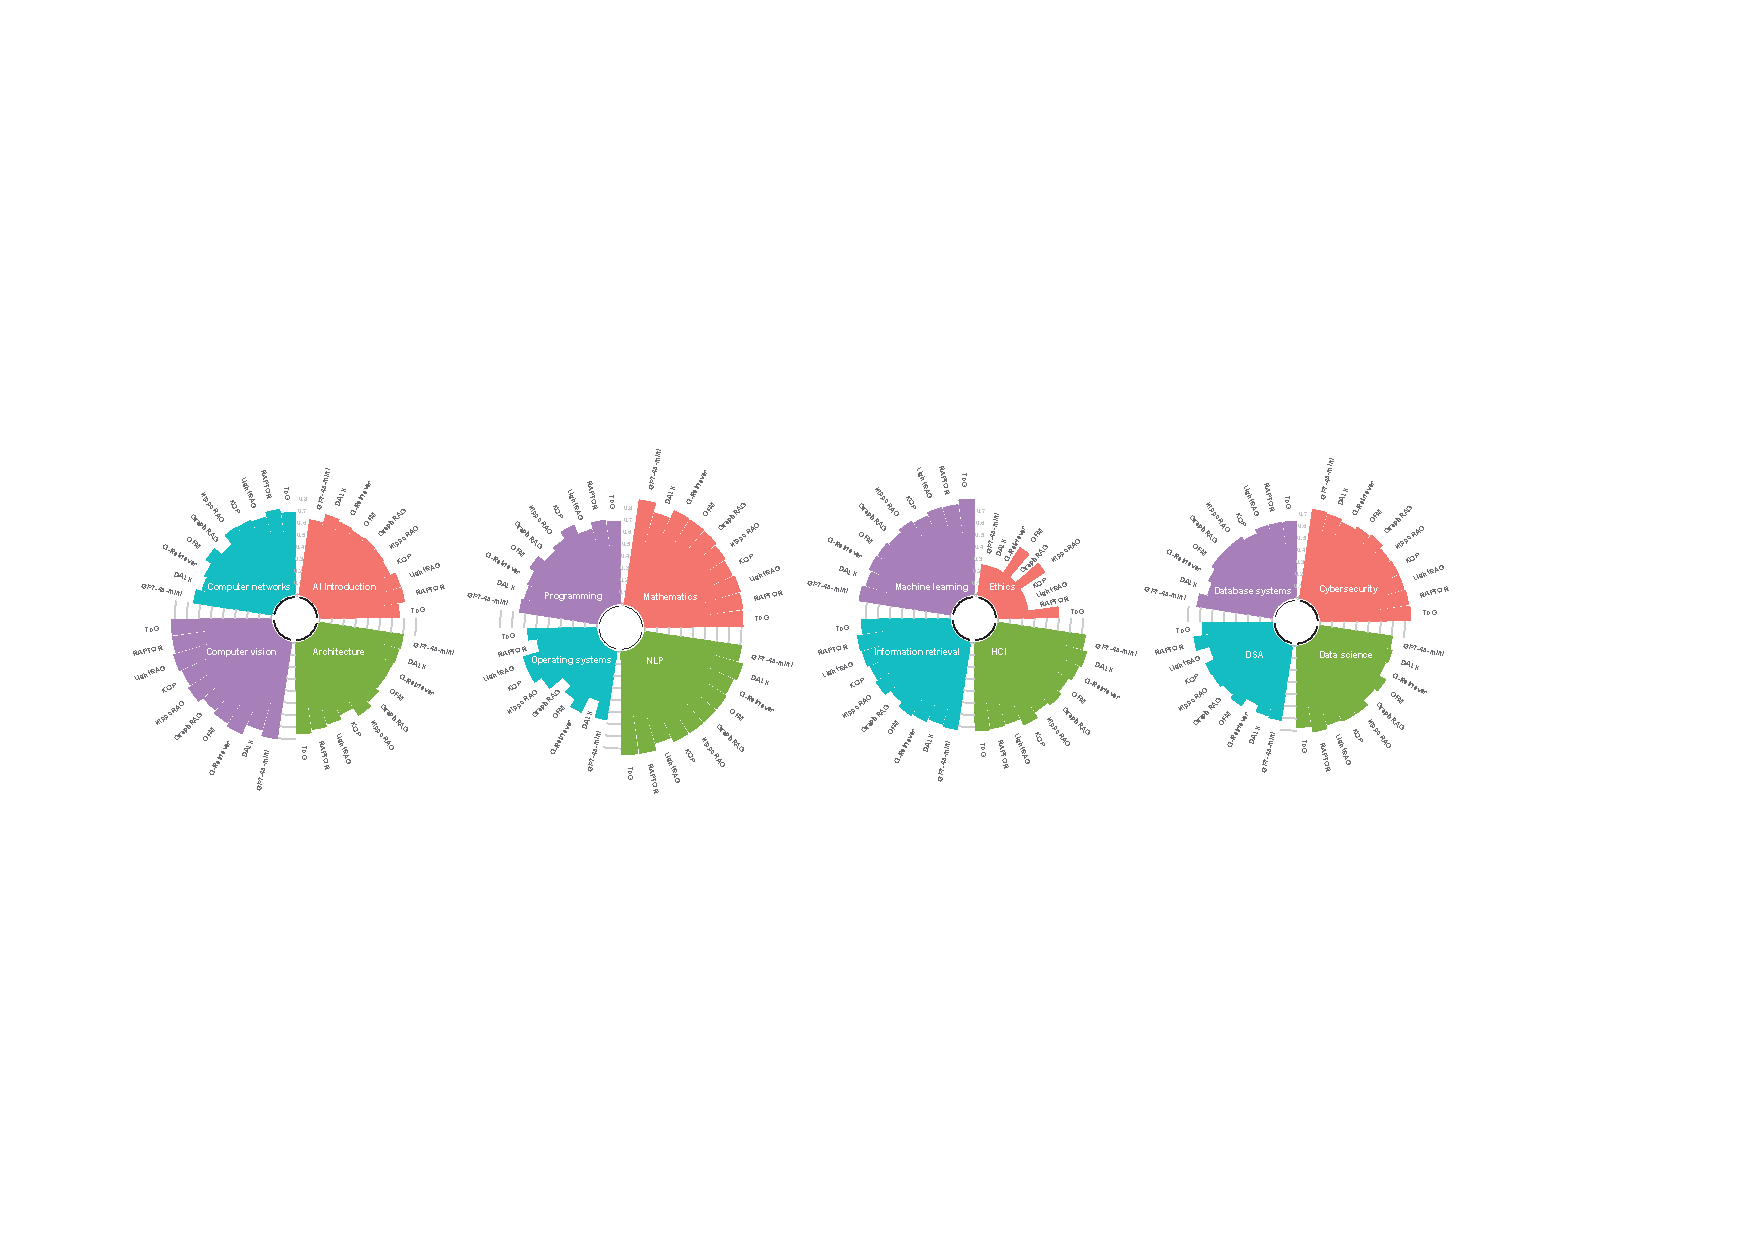
\includegraphics[width=\linewidth]{topic_4.pdf}
    \caption{Comparison of Generation Accuracy by Topic.}
    \label{fig:generation}
\end{figure*}
% \vspace{-10pt}
\subsection{Observation}
% \subsection{Can GraphRAG improve performance across all question types?}
\textit{\textbf{`Can GraphRAG improve performance across all question types?'}}

\textbf{Accuracy drop of MC questions.} LLMs have internalized vast amounts of knowledge through extensive training on large corpora, enabling them to often correctly select answers in multiple-choice tasks. However, GraphRAG’s retrieval-based augmentation may introduce redundant or loosely related information that does not precisely match the question context. Such retrieval noise can interfere with the model’s decision-making ability, ultimately reducing its accuracy on MC questions.

\textbf{Improvement in TF questions.} TF questions require binary judgments about factual or logical statements. LLMs may contain blind spots or incomplete knowledge for certain facts, leading to incorrect answers. By retrieving relevant factual evidence, GraphRAG helps the model verify statements before answering. These supplementals improve the model’s accuracy on TF questions.

\textbf{Improvement in OE questions.} Open-ended questions allow for expansive, detailed responses, which can be challenging for LLMs that rely solely on their internal knowledge. GraphRAG mitigates this challenge by providing additional context and facts from external corpora. The retrieved information enriches the model’s responses, improves subject-matter detail and expressiveness, and reduces instances of hallucination by grounding answers in explicit evidence.

\textbf{Different effects in FB \& MS questions.} Fill-in-blank questions demand precise contextual understanding to correctly predict missing words. GraphRAG’s retrieved corpora often fail to match exact contexts, introducing noise that degrades the model’s performance on FB questions. Multi-select questions require choosing multiple correct answers from a set and involve reasoning over complex combinations of options; if GraphRAG’s retrieval omits relevant answer options or includes irrelevant details, it can confuse the model. As a result, these question types place high demands on retrieval precision; GraphRAG may have limited benefit unless its retrieval is highly accurate.

% \subsection{Can GraphRAG effectively enhance LLMs’ reasoning ability?}
\textit{\textbf{`Can GraphRAG effectively enhance LLMs’ reasoning ability?'}}

Experiments demonstrate that GraphRAG effectively enhances the reasoning capabilities of LLMs across diverse question types, increasing the probability of generating correct rationales alongside answers. This is attributed to their efficient retrieval mechanisms, which not only identify highly relevant corpora for questions but also provide robust evidential support for LLM reasoning processes. In particular, existing benchmarks lack systematic evaluation of GraphRAG's reasoning capabilities, an aspect of critical importance in real-world applications. For example, in the college-level educational context targeted in this document, users seeking professional knowledge expect not only correct answers, but also explicit rationales to facilitate understanding and knowledge acquisition. Similarly, in medical scenarios, patients require clear rationales for medication along with treatment recommendations to ensure transparency in decision-making. Thus, an effective GraphRAG approach should aim not only for high accuracy in answer generation but also for strong reasoning and explainability. 
% Providing clear evidence-based justifications and reasoning chains is essential for meeting the requirements of explainability and transparency in real-world scenarios.

\begin{figure*}[htbp]
    \centering
    
\includegraphics[width=0.8\linewidth]{case_study.pdf}
    \caption{A case study in the topic of computer networks.}
    \label{fig:case_study}
\end{figure*}
% \vspace{-20pt}

\subsection{Case Study}
As illustrated in Fig~\ref{fig:case_study}, we present a case study highlighting specific challenges within our dataset. Our questions span 16 core topics in undergraduate computer science; here, we focus on a sample from the Computer Networks section. This example demonstrates that (i) the questions demand specialized, college-level knowledge, and (ii) the correct answer cannot be retrieved through simple lookup. Instead, solving the problem requires synthesizing multiple reasoning steps to construct a coherent rationale before generating the final answer.
\section{Conclusion}
In this paper, we present GraphRAG-Bench, the first domain-specific benchmark designed for GraphRAG, comprising a 16-discipline dataset that challenges methods with multi-hop reasoning, complex algorithmic/programming tasks, mathematical computing, and varied question types. Our comprehensive, multi-dimensional evaluation, spanning graph construction, knowledge retrieval, generation and reasoning, quantifies the enhancement of LLM reasoning when augmented with structured knowledge. Extensive experiments on nine state-of-the-art GraphRAG methods reveal the significant role of graph integration in improving reasoning and generation performance.
% \section{Conclusion }

\medskip

\newpage
{
\small
\bibliographystyle{ieeetr}  % abbrv, named
\bibliography{ref}
}


%%%%%%%%%%%%%%%%%%%%%%%%%%%%%%%%%%%%%%%%%%%%%%%%%%%%%%%%%%%%
% \clearpage
% \appendix
% \section{Additional experiments}
% \subsection{Topic‐specific reasoning analysis}
% \begin{figure*}[htbp]
%     \centering
%     \includegraphics[width=\linewidth]{topic_4_Rationale.pdf}
%     \caption{Comparison of R score by Topic.}
%     \label{fig:R score}
% \end{figure*}
% Given that our dataset encompasses 16 thematic domains, we conducted experiments to analyze the reasoning capabilities of GraphRAG across different topics. Results indicate that the large language model (LLM) based on GPT-4o-mini demonstrates significant improvements in reasoning through GraphRAG across most domains. However, the following intriguing observations were made:

% \textbf{Operating System Domain.} The LLM exhibits suboptimal performance in this domain. While GraphRAG provides marginal improvements in reasoning capabilities, overall scores remain low. This is primarily attributed to the highly specialized, systematic, and logically complex nature of operating system knowledge, which involves multi-layered principles such as process scheduling, memory management, and file systems, requiring precise grasp of conceptual definitions, algorithmic workflows, and causal relationships between entities. General-purpose training data for LLMs often lack comprehensive coverage of such granular knowledge systems, and the models themselves have inherent limitations in structured logical reasoning.

% \textbf{Ethics Domain.} Consistent with the generation accuracy results, LLMs face substantial challenges in reasoning about ethical questions. Ethical problems fundamentally involve subjective value judgments, whose meanings are rooted in dynamic contexts of moral trade-offs and social norms. The symbolic representations captured by LLMs through statistical learning struggle to accurately model ambiguous ethical constructs, leading to intrinsic difficulties in both generating correct answers and constructing valid reasoning chains.

% \begin{figure*}[htbp]
%     \centering
%     \includegraphics[width=\linewidth]{topic_4_Rationale.pdf}
%     \caption{Comparison of AR score by Topic.}
%     \label{fig:AR score}
% \end{figure*}

% We further evaluated the AR scores of GraphRAG across different topics. Experimental results show that AR scores generally align with R scores in most cases. However, a notable observation emerges in the database systems domain: AR scores are significantly lower than R scores, indicating a high prevalence of "correct reasoning but incorrect answering" in LLMs, where reasoning steps diverge from final answer generation. This discrepancy arises because database system problems require models to reference specialized concepts such as relational algebra operations, transaction isolation levels, ACID properties, and query optimizer cost models, yet models do not perform formal computations or analyze critical factors like underlying data distribution and index selectivity. Although models may decompose processes like schema design or concurrency control according to human logical paradigms in chain-of-thought reasoning, their token selection during answer generation prioritizes statistical fluency from training corpora over contextual logical accuracy. The strict requirements for precise logical operations (e.g., cost estimation, deadlock detection) in database tasks create a fundamental mismatch with the model’s learned fuzzy statistical patterns from general text, leading to reasoning chains that appear plausible in intermediate steps but produce erroneous conclusions at technical junctures, such as failing to execute physical query optimization calculations, due to the absence of real-world logical validation.
% \subsection{Compute resources}
% All code is done in Python, and experiments are conducted on H100*2 GPUs.
% \section{Metrics details}
% \textbf{Prompt of OE and FB questions.}

% Fig.~\ref{fig:prompt_gen} is the prompt used to generate the LLM-judge score for OE and FB questions.
% \begin{figure*}[htbp]
%     \centering
%     \includegraphics[width=\linewidth]{prompt_gen.pdf}
%     \caption{Prompt of generation grading for OE and FB questions.}
%     \label{fig:prompt_gen}
% \end{figure*}

% \textbf{Prompt of reasoning grading.}

% Fig.~\ref{fig:prompt_rationale} is the prompt used to evaluate the reasoning score R.

% \begin{figure*}[htbp]
%     \centering
%     \includegraphics[width=\linewidth]{prompt_rationale.pdf}
%     \caption{Prompt of rationale grading.}
%     \label{fig:prompt_rationale}
% \end{figure*}

% \textbf{Details of AR score.}

% The AR score is computed based on the combination of answer correctness (generation score) and rationale correctness (reasoning score), with the following evaluation rules:
% \begin{itemize}
%     \item When both the answer and rationale are fully correct (generation score = 1 and reasoning score = 1), the AR score is 1.0.
%     \item If the answer is correct but the rationale is partially correct (generation score = 1 and reasoning score = 0.5), the AR score is 0.5.
%     \item When the answer is correct but the rationale is incorrect (generation score = 1 and reasoning score = 0), the AR score is 0.0.
%     \item For incorrect answers with a fully correct rationale (generation score = 0 and reasoning score = 1), the AR score is 0.5.
%     \item If both the answer is incorrect and the rationale is partially correct (generation score = 0 and reasoning score = 0.5), the AR score is 0.25.
%     \item In all other cases (e.g., incorrect answer with incorrect or missing rationale), the AR score is 0.0.
% \end{itemize}
% This scoring scheme systematically captures the alignment between answers and their supporting reasoning, emphasizing the importance of both correctness and logical consistency in evaluating model performance.
% \section{Limitations of Existing GraphRAG Datasets}
% Through a systematic review of benchmark datasets used by contemporary Graph-RAG methods, we have identified four critical limitations that undermine both task suitability and the validity of evaluation results:

% \textbf{Superficial retrieval tasks.}  
%     Most datasets pose questions that can be answered by straightforward text retrieval, without requiring deep integration of graph structure or sophisticated semantic reasoning. Consequently, models may achieve high scores by exploiting shallow keyword matching, offering no insight into their true capabilities in relational reasoning or entity-association modeling.

% \textbf{Synthetic and unrepresentative queries.}  
%     Questions are typically generated via hand-crafted rules, yielding simplified language that lacks the domain-specific terminology, ambiguous intent, and syntactic variety found in real user queries. This synthetic distribution diverges sharply from natural problem settings, limiting the ecological validity of any conclusions about model generalization.

% \textbf{Cross-task misalignment.}  
%     Many datasets are inherited from disparate tasks (e.g., knowledge-graph question answering) whose annotation schemes and answer formats do not align with the core objectives of Graph-RAG—namely, constructing and leveraging heterogeneous graph structures to guide multi-source information fusion. Transferring evaluation metrics across tasks therefore introduces inconsistencies that dilute the relevance of experimental findings for advancing Graph-RAG techniques.

% \textbf{Opaque reasoning evaluation.}  
%     Existing benchmarks supply only final answers or explicit node sequences, but omit any structural or narrative annotation of the underlying inference process. Key decision points—such as why a particular graph subpath was selected or how evidence from multiple sources is reconciled—remain unexamined. Without annotated rationales, evaluation reduces to binary correctness checks and cannot assess a model’s genuine reasoning competence.

% These limitations collectively motivate the design of a dedicated benchmark that both challenges Graph-RAG models on core reasoning skills and provides richly structured annotations for fine-grained, interpretability-driven evaluation. 
% \section{Limitations of this paper}
% Despite the valuable contributions of this study, we acknowledge its limitations:  (1) Our dataset currently only contains English content; more detailed research should be done in the future for different languages. (2) Other modal data such as images are not included in the current data set, and richer multimodal datasets can be considered in the future.

% %%%%%%%%%%%%%%%%%%%%%%%%%%%%%%%%%%%%%%%%%%%%%%%%%%%%%%%%%%%

% \newpage
% \section*{NeurIPS Paper Checklist}
% \begin{enumerate}

% \item {\bf Claims}
%     \item[] Question: Do the main claims made in the abstract and introduction accurately reflect the paper's contributions and scope?
%     \item[] Answer: \answerYes{} % Replace by \answerYes{}, \answerNo{}, or \answerNA{}.
%     \item[] Justification: The main claims in the abstract and introduction precisely outline the paper's core contributions and scope, aligning with the theoretical analysis and experimental results.
%     \item[] Guidelines:
%     \begin{itemize}
%         \item The answer NA means that the abstract and introduction do not include the claims made in the paper.
%         \item The abstract and/or introduction should clearly state the claims made, including the contributions made in the paper and important assumptions and limitations. A No or NA answer to this question will not be perceived well by the reviewers. 
%         \item The claims made should match theoretical and experimental results, and reflect how much the results can be expected to generalize to other settings. 
%         \item It is fine to include aspirational goals as motivation as long as it is clear that these goals are not attained by the paper. 
%     \end{itemize}

% \item {\bf Limitations}
%     \item[] Question: Does the paper discuss the limitations of the work performed by the authors?
%     \item[] Answer: \answerYes{} % Replace by \answerYes{}, \answerNo{}, or \answerNA{}.
%     \item[] Justification: The paper includes a dedicated "Limitations" section in appendix that candidly discusses the limitations of this work.
%     \item[] Guidelines:
%     \begin{itemize}
%         \item The answer NA means that the paper has no limitation while the answer No means that the paper has limitations, but those are not discussed in the paper. 
%         \item The authors are encouraged to create a separate "Limitations" section in their paper.
%         \item The paper should point out any strong assumptions and how robust the results are to violations of these assumptions (e.g., independence assumptions, noiseless settings, model well-specification, asymptotic approximations only holding locally). The authors should reflect on how these assumptions might be violated in practice and what the implications would be.
%         \item The authors should reflect on the scope of the claims made, e.g., if the approach was only tested on a few datasets or with a few runs. In general, empirical results often depend on implicit assumptions, which should be articulated.
%         \item The authors should reflect on the factors that influence the performance of the approach. For example, a facial recognition algorithm may perform poorly when image resolution is low or images are taken in low lighting. Or a speech-to-text system might not be used reliably to provide closed captions for online lectures because it fails to handle technical jargon.
%         \item The authors should discuss the computational efficiency of the proposed algorithms and how they scale with dataset size.
%         \item If applicable, the authors should discuss possible limitations of their approach to address problems of privacy and fairness.
%         \item While the authors might fear that complete honesty about limitations might be used by reviewers as grounds for rejection, a worse outcome might be that reviewers discover limitations that aren't acknowledged in the paper. The authors should use their best judgment and recognize that individual actions in favor of transparency play an important role in developing norms that preserve the integrity of the community. Reviewers will be specifically instructed to not penalize honesty concerning limitations.
%     \end{itemize}

% \item {\bf Theory assumptions and proofs}
%     \item[] Question: For each theoretical result, does the paper provide the full set of assumptions and a complete (and correct) proof?
%     \item[] Answer: \answerNA{} % Replace by \answerYes{}, \answerNo{}, or \answerNA{}.
%     \item[] Justification: The paper does not include theorems and formulas. It is a benchmark and dataset paper.
%     \item[] Guidelines:
%     \begin{itemize}
%         \item The answer NA means that the paper does not include theoretical results. 
%         \item All the theorems, formulas, and proofs in the paper should be numbered and cross-referenced.
%         \item All assumptions should be clearly stated or referenced in the statement of any theorems.
%         \item The proofs can either appear in the main paper or the supplemental material, but if they appear in the supplemental material, the authors are encouraged to provide a short proof sketch to provide intuition. 
%         \item Inversely, any informal proof provided in the core of the paper should be complemented by formal proofs provided in appendix or supplemental material.
%         \item Theorems and Lemmas that the proof relies upon should be properly referenced. 
%     \end{itemize}

%     \item {\bf Experimental result reproducibility}
%     \item[] Question: Does the paper fully disclose all the information needed to reproduce the main experimental results of the paper to the extent that it affects the main claims and/or conclusions of the paper (regardless of whether the code and data are provided or not)?
%     \item[] Answer: \answerYes{} % Replace by \answerYes{}, \answerNo{}, or \answerNA{}.
%     \item[] Justification: The paper provides detailed descriptions of experimental protocols, hyperparameters and evaluation metrics, enabling reproduction of main results; Dataset is also submitted.
%     \item[] Guidelines:
%     \begin{itemize}
%         \item The answer NA means that the paper does not include experiments.
%         \item If the paper includes experiments, a No answer to this question will not be perceived well by the reviewers: Making the paper reproducible is important, regardless of whether the code and data are provided or not.
%         \item If the contribution is a dataset and/or model, the authors should describe the steps taken to make their results reproducible or verifiable. 
%         \item Depending on the contribution, reproducibility can be accomplished in various ways. For example, if the contribution is a novel architecture, describing the architecture fully might suffice, or if the contribution is a specific model and empirical evaluation, it may be necessary to either make it possible for others to replicate the model with the same dataset, or provide access to the model. In general. releasing code and data is often one good way to accomplish this, but reproducibility can also be provided via detailed instructions for how to replicate the results, access to a hosted model (e.g., in the case of a large language model), releasing of a model checkpoint, or other means that are appropriate to the research performed.
%         \item While NeurIPS does not require releasing code, the conference does require all submissions to provide some reasonable avenue for reproducibility, which may depend on the nature of the contribution. For example
%         \begin{enumerate}
%             \item If the contribution is primarily a new algorithm, the paper should make it clear how to reproduce that algorithm.
%             \item If the contribution is primarily a new model architecture, the paper should describe the architecture clearly and fully.
%             \item If the contribution is a new model (e.g., a large language model), then there should either be a way to access this model for reproducing the results or a way to reproduce the model (e.g., with an open-source dataset or instructions for how to construct the dataset).
%             \item We recognize that reproducibility may be tricky in some cases, in which case authors are welcome to describe the particular way they provide for reproducibility. In the case of closed-source models, it may be that access to the model is limited in some way (e.g., to registered users), but it should be possible for other researchers to have some path to reproducing or verifying the results.
%         \end{enumerate}
%     \end{itemize}


% \item {\bf Open access to data and code}
%     \item[] Question: Does the paper provide open access to the data and code, with sufficient instructions to faithfully reproduce the main experimental results, as described in supplemental material?
%     \item[] Answer: \answerYes{} % Replace by \answerYes{}, \answerNo{}, or \answerNA{}.
%     \item[] Justification:The paper provides the dataset proposed.
%     \item[] Guidelines:
%     \begin{itemize}
%         \item The answer NA means that paper does not include experiments requiring code.
%         \item Please see the NeurIPS code and data submission guidelines (\url{https://nips.cc/public/guides/CodeSubmissionPolicy}) for more details.
%         \item While we encourage the release of code and data, we understand that this might not be possible, so “No” is an acceptable answer. Papers cannot be rejected simply for not including code, unless this is central to the contribution (e.g., for a new open-source benchmark).
%         \item The instructions should contain the exact command and environment needed to run to reproduce the results. See the NeurIPS code and data submission guidelines (\url{https://nips.cc/public/guides/CodeSubmissionPolicy}) for more details.
%         \item The authors should provide instructions on data access and preparation, including how to access the raw data, preprocessed data, intermediate data, and generated data, etc.
%         \item The authors should provide scripts to reproduce all experimental results for the new proposed method and baselines. If only a subset of experiments are reproducible, they should state which ones are omitted from the script and why.
%         \item At submission time, to preserve anonymity, the authors should release anonymized versions (if applicable).
%         \item Providing as much information as possible in supplemental material (appended to the paper) is recommended, but including URLs to data and code is permitted.
%     \end{itemize}


% \item {\bf Experimental setting/details}
%     \item[] Question: Does the paper specify all the training and test details (e.g., data splits, hyperparameters, how they were chosen, type of optimizer, etc.) necessary to understand the results?
%     \item[] Answer: \answerYes{} % Replace by \answerYes{}, \answerNo{}, or \answerNA{}.
%     \item[] Justification: The paper specifies all the details, such as hyperparameters and base LLM, etc.
%     \item[] Guidelines:
%     \begin{itemize}
%         \item The answer NA means that the paper does not include experiments.
%         \item The experimental setting should be presented in the core of the paper to a level of detail that is necessary to appreciate the results and make sense of them.
%         \item The full details can be provided either with the code, in appendix, or as supplemental material.
%     \end{itemize}

% \item {\bf Experiment statistical significance}
%     \item[] Question: Does the paper report error bars suitably and correctly defined or other appropriate information about the statistical significance of the experiments?
%     \item[] Answer: \answerNA{} % Replace by \answerYes{}, \answerNo{}, or \answerNA{}.
%     \item[] Justification: The experiments are not related to statistical significance.
%     \item[] Guidelines:
%     \begin{itemize}
%         \item The answer NA means that the paper does not include experiments.
%         \item The authors should answer "Yes" if the results are accompanied by error bars, confidence intervals, or statistical significance tests, at least for the experiments that support the main claims of the paper.
%         \item The factors of variability that the error bars are capturing should be clearly stated (for example, train/test split, initialization, random drawing of some parameter, or overall run with given experimental conditions).
%         \item The method for calculating the error bars should be explained (closed form formula, call to a library function, bootstrap, etc.)
%         \item The assumptions made should be given (e.g., Normally distributed errors).
%         \item It should be clear whether the error bar is the standard deviation or the standard error of the mean.
%         \item It is OK to report 1-sigma error bars, but one should state it. The authors should preferably report a 2-sigma error bar than state that they have a 96\% CI, if the hypothesis of Normality of errors is not verified.
%         \item For asymmetric distributions, the authors should be careful not to show in tables or figures symmetric error bars that would yield results that are out of range (e.g. negative error rates).
%         \item If error bars are reported in tables or plots, The authors should explain in the text how they were calculated and reference the corresponding figures or tables in the text.
%     \end{itemize}

% \item {\bf Experiments compute resources}
%     \item[] Question: For each experiment, does the paper provide sufficient information on the computer resources (type of compute workers, memory, time of execution) needed to reproduce the experiments?
%     \item[] Answer: \answerYes{} % Replace by \answerYes{}, \answerNo{}, or \answerNA{}.
%     \item[] Justification: We provide it in the supplementary materials.
%     \item[] Guidelines:
%     \begin{itemize}
%         \item The answer NA means that the paper does not include experiments.
%         \item The paper should indicate the type of compute workers CPU or GPU, internal cluster, or cloud provider, including relevant memory and storage.
%         \item The paper should provide the amount of compute required for each of the individual experimental runs as well as estimate the total compute. 
%         \item The paper should disclose whether the full research project required more compute than the experiments reported in the paper (e.g., preliminary or failed experiments that didn't make it into the paper). 
%     \end{itemize}
    
% \item {\bf Code of ethics}
%     \item[] Question: Does the research conducted in the paper conform, in every respect, with the NeurIPS Code of Ethics \url{https://neurips.cc/public/EthicsGuidelines}?
%     \item[] Answer: \answerYes{} % Replace by \answerYes{}, \answerNo{}, or \answerNA{}.
%     \item[] Justification: The research conforms with the NeurIPS Code of Ethics in every respect.
%     \item[] Guidelines:
%     \begin{itemize}
%         \item The answer NA means that the authors have not reviewed the NeurIPS Code of Ethics.
%         \item If the authors answer No, they should explain the special circumstances that require a deviation from the Code of Ethics.
%         \item The authors should make sure to preserve anonymity (e.g., if there is a special consideration due to laws or regulations in their jurisdiction).
%     \end{itemize}


% \item {\bf Broader impacts}
%     \item[] Question: Does the paper discuss both potential positive societal impacts and negative societal impacts of the work performed?
%     \item[] Answer: \answerYes{} % Replace by \answerYes{}, \answerNo{}, or \answerNA{}.
%     \item[] Justification: We have discussed in the paper that this research will have a great positive impact on the field of education.
%     \item[] Guidelines:
%     \begin{itemize}
%         \item The answer NA means that there is no societal impact of the work performed.
%         \item If the authors answer NA or No, they should explain why their work has no societal impact or why the paper does not address societal impact.
%         \item Examples of negative societal impacts include potential malicious or unintended uses (e.g., disinformation, generating fake profiles, surveillance), fairness considerations (e.g., deployment of technologies that could make decisions that unfairly impact specific groups), privacy considerations, and security considerations.
%         \item The conference expects that many papers will be foundational research and not tied to particular applications, let alone deployments. However, if there is a direct path to any negative applications, the authors should point it out. For example, it is legitimate to point out that an improvement in the quality of generative models could be used to generate deepfakes for disinformation. On the other hand, it is not needed to point out that a generic algorithm for optimizing neural networks could enable people to train models that generate Deepfakes faster.
%         \item The authors should consider possible harms that could arise when the technology is being used as intended and functioning correctly, harms that could arise when the technology is being used as intended but gives incorrect results, and harms following from (intentional or unintentional) misuse of the technology.
%         \item If there are negative societal impacts, the authors could also discuss possible mitigation strategies (e.g., gated release of models, providing defenses in addition to attacks, mechanisms for monitoring misuse, mechanisms to monitor how a system learns from feedback over time, improving the efficiency and accessibility of ML).
%     \end{itemize}
    
% \item {\bf Safeguards}
%     \item[] Question: Does the paper describe safeguards that have been put in place for responsible release of data or models that have a high risk for misuse (e.g., pretrained language models, image generators, or scraped datasets)?
%     \item[] Answer: \answerNA{} % Replace by \answerYes{}, \answerNo{}, or \answerNA{}.
%     \item[] Justification: The paper poses no such risks.
%     \item[] Guidelines:
%     \begin{itemize}
%         \item The answer NA means that the paper poses no such risks.
%         \item Released models that have a high risk for misuse or dual-use should be released with necessary safeguards to allow for controlled use of the model, for example by requiring that users adhere to usage guidelines or restrictions to access the model or implementing safety filters. 
%         \item Datasets that have been scraped from the Internet could pose safety risks. The authors should describe how they avoided releasing unsafe images.
%         \item We recognize that providing effective safeguards is challenging, and many papers do not require this, but we encourage authors to take this into account and make a best faith effort.
%     \end{itemize}

% \item {\bf Licenses for existing assets}
%     \item[] Question: Are the creators or original owners of assets (e.g., code, data, models), used in the paper, properly credited and are the license and terms of use explicitly mentioned and properly respected?
%     \item[] Answer: \answerYes{} % Replace by \answerYes{}, \answerNo{}, or \answerNA{}.
%     \item[] Justification: Please refer to supplementary materials.
%     \item[] Guidelines:
%     \begin{itemize}
%         \item The answer NA means that the paper does not use existing assets.
%         \item The authors should cite the original paper that produced the code package or dataset.
%         \item The authors should state which version of the asset is used and, if possible, include a URL.
%         \item The name of the license (e.g., CC-BY 4.0) should be included for each asset.
%         \item For scraped data from a particular source (e.g., website), the copyright and terms of service of that source should be provided.
%         \item If assets are released, the license, copyright information, and terms of use in the package should be provided. For popular datasets, \url{paperswithcode.com/datasets} has curated licenses for some datasets. Their licensing guide can help determine the license of a dataset.
%         \item For existing datasets that are re-packaged, both the original license and the license of the derived asset (if it has changed) should be provided.
%         \item If this information is not available online, the authors are encouraged to reach out to the asset's creators.
%     \end{itemize}

% \item {\bf New assets}
%     \item[] Question: Are new assets introduced in the paper well documented and is the documentation provided alongside the assets?
%     \item[] Answer: \answerYes{} % Replace by \answerYes{}, \answerNo{}, or \answerNA{}.
%     \item[] Justification: Please refer to supplementary materials.
%     \item[] Guidelines:
%     \begin{itemize}
%         \item The answer NA means that the paper does not release new assets.
%         \item Researchers should communicate the details of the dataset/code/model as part of their submissions via structured templates. This includes details about training, license, limitations, etc. 
%         \item The paper should discuss whether and how consent was obtained from people whose asset is used.
%         \item At submission time, remember to anonymize your assets (if applicable). You can either create an anonymized URL or include an anonymized zip file.
%     \end{itemize}

% \item {\bf Crowdsourcing and research with human subjects}
%     \item[] Question: For crowdsourcing experiments and research with human subjects, does the paper include the full text of instructions given to participants and screenshots, if applicable, as well as details about compensation (if any)? 
%     \item[] Answer: \answerNA{} % Replace by \answerYes{}, \answerNo{}, or \answerNA{}.
%     \item[] Justification: The paper does not involve crowdsourcing or research with human subjects.
%     \item[] Guidelines:
%     \begin{itemize}
%         \item The answer NA means that the paper does not involve crowdsourcing nor research with human subjects.
%         \item Including this information in the supplemental material is fine, but if the main contribution of the paper involves human subjects, then as much detail as possible should be included in the main paper. 
%         \item According to the NeurIPS Code of Ethics, workers involved in data collection, curation, or other labor should be paid at least the minimum wage in the country of the data collector. 
%     \end{itemize}

% \item {\bf Institutional review board (IRB) approvals or equivalent for research with human subjects}
%     \item[] Question: Does the paper describe potential risks incurred by study participants, whether such risks were disclosed to the subjects, and whether Institutional Review Board (IRB) approvals (or an equivalent approval/review based on the requirements of your country or institution) were obtained?
%     \item[] Answer: \answerNA{} % Replace by \answerYes{}, \answerNo{}, or \answerNA{}.
%     \item[] Justification: The paper does not involve research with human subjects or crowdsourcing.
%     \item[] Guidelines:
%     \begin{itemize}
%         \item The answer NA means that the paper does not involve crowdsourcing nor research with human subjects.
%         \item Depending on the country in which research is conducted, IRB approval (or equivalent) may be required for any human subjects research. If you obtained IRB approval, you should clearly state this in the paper. 
%         \item We recognize that the procedures for this may vary significantly between institutions and locations, and we expect authors to adhere to the NeurIPS Code of Ethics and the guidelines for their institution. 
%         \item For initial submissions, do not include any information that would break anonymity (if applicable), such as the institution conducting the review.
%     \end{itemize}

% \item {\bf Declaration of LLM usage}
%     \item[] Question: Does the paper describe the usage of LLMs if it is an important, original, or non-standard component of the core methods in this research? Note that if the LLM is used only for writing, editing, or formatting purposes and does not impact the core methodology, scientific rigorousness, or originality of the research, declaration is not required.
%     %this research? 
%     \item[] Answer: \answerNA{} % Replace by \answerYes{}, \answerNo{}, or \answerNA{}.
%     \item[] Justification: LLMs is not applied to any original content about the manuscript.
%     \item[] Guidelines:
%     \begin{itemize}
%         \item The answer NA means that the core method development in this research does not involve LLMs as any important, original, or non-standard components.
%         \item Please refer to our LLM policy (\url{https://neurips.cc/Conferences/2025/LLM}) for what should or should not be described.
%     \end{itemize}

% \end{enumerate}


\end{document}